% Author: Marek Fiser <tikz at marekfiser.cz>
% MESIF protocol: http://en.wikipedia.org/wiki/MESIF_protocol
%Template found online and modified to fit specific needs
\documentclass[tikz, border=10pt]{standalone}
\usetikzlibrary{arrows}
\begin{document}
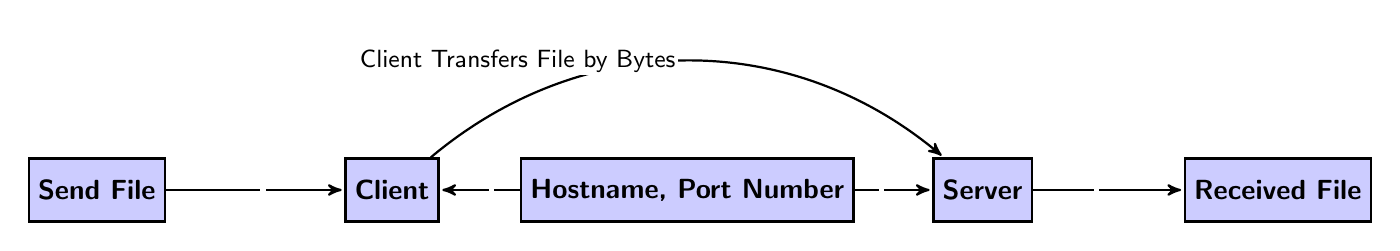
\begin{tikzpicture}[->,>=stealth',shorten >=1pt,auto,node distance=3.75cm,
  thick,main node/.style={rectangle,fill=blue!20,draw,
  font=\sffamily\bfseries,minimum size=8mm}]

  \node[main node] (HP) {Hostname, Port Number};
  \node[main node] (C) [left of=HP] {Client};
  \node[main node] (S) [right of=HP] {Server};
  \node[main node] (SF) [left of=C] {Send File};
  \node[main node] (RF) [right of=S] {Received File};

  \path[every node/.style={font=\sffamily\small,
  		fill=white,inner sep=1pt}]
  		
  	%Shows Send file taken as parameter for Client
  	(SF) edge [left=20] node[right=.5mm] {} (C)
    
    %Shows request and reply between client and server%
    (C) edge [bend left=40] node[left=1mm] {Client Transfers File by Bytes} (S)
    %No information is sent back from Server
    %(S) edge [bend left=40] node[right=1mm] {} (C)
    (S) edge [right=40] node[left=1mm] {} (RF)
    
    
    %Shows connection between client and server through hostname and port number
    (HP) edge node[left=1mm] {} (S)
    (HP) edge node[right=1mm] {} (C);
	
\end{tikzpicture}
\end{document}\textsl{•}